\section{Case study: the sparse-attention indexer}
\label{sec:indexer}
Long prompts take minutes on a laptop, and part of that time goes to the indexer. For a query with indexer heads $\q_1,\dots,\q_H\in\RR^{d}$ and signed head weights $w_1,\dots,w_H$, the reference scores each visible compressed key $\kv_j$ as
\begin{equation}
s_j \;=\; \bfround\!\Big(\sum_{h=1}^{H} \bfround\big(\relu{\bfround(\q_h^\top\kv_j)}\, w_h\big)\Big),
\label{eq:score}
\end{equation}
with the outer sum accumulated in FP32, and keeps the best $K$ keys. Prefill scores every query against every visible key, so this cost grows with the square of the prompt length. We tried two ways to make it cheaper. The first computes Equation~\eqref{eq:score} faster without changing any result, and the second skips keys that cannot make the cut.

\subsection{Faster scoring with the same results}
\paragraph{BF16 products.} The reference computes each product $\q_h^\top\kv_j$ in FP32 and then rounds it to BF16. Both inputs are FP4 values with power-of-two scales, which BF16 represents exactly, and the following lemma shows when a BF16 matrix multiplication returns the same rounded result.
\begin{lemma}
\label{lem:exact}
Let $\q,\kv\in\RR^{128}$ hold E2M1 values with one power-of-two scale per block of 32 elements, and let $\sigma_b$ be the product of the two scales of block $b$. Assume that $\max_b\sigma_b/\min_b\sigma_b\le 2^{9}$ and that every block product stays in the normal FP32 range. Then every partial sum of $\q^\top\kv$, in any order, is exactly representable in FP32, and a BF16 matrix multiplication that accumulates in FP32 and rounds once returns $\bfround(\q^\top\kv)$, the reference result.
\end{lemma}
The appendix gives the proof. MLX's BF16 matrix kernels accumulate in FP32, although we checked this empirically rather than for every kernel variant. Where the scale condition fails, both computations are ordinary FP32 sums whose last bit can depend on the order of summation, just as it can between different GPU kernels running the reference. On indexer inputs captured from a real 32K-token prompt, the BF16 version reproduced every one of about a billion scores.

\paragraph{Fused head reduction.} After the matrix multiplication, Equation~\eqref{eq:score} still needs a ReLU, a weighting and a rounding for every element, followed by a sum over heads. Written as array operations, this reads a large intermediate tensor three times. We replaced it with a single Metal kernel in which each thread handles one pair of query and key and walks over the heads, applying the same roundings in the same order. On every input we tested it matches the array version. Both sum the heads in FP32, so their results could differ in the last bit only if the summation orders differed and the terms spanned a very wide range, which is equally true of the reference. Figure~\ref{fig:indexer}a shows that together the two changes make an indexer block about twice as fast on real inputs, with the same selected keys.

\paragraph{Fixed tie order.} A partition-based Top-$K$ leaves ties at the boundary to the kernel. We sort by a 64-bit key built from the BF16 score and the position, so that ties go to the earlier position and a NaN score is never selected. Selection thereby becomes a pure function of the scores, which an exact screening method must also reproduce.

\subsection{Skipping keys: exact screening}
\label{sec:dosa}
DoSA \citep{dosa} skips keys while keeping the selection exact. A seed set of keys gives a lower bound $\tau$ on the $K$-th best score, a cheap upper bound $U_j$ is computed for every other key, and keys with $U_j<\tau$ are dropped before full scoring. DoSA reports large speed-ups on GLM-5.2 and DeepSeek-V3.2 at contexts of half a million tokens and more. V4.1-Flash differs in three ways that could matter: it has fewer indexer heads, a smaller $K$, and its own two-level candidate selection. We therefore measured how well such a bound works on this model.

\paragraph{Setup.} We captured the indexer inputs of a real 32K-token prompt and studied every index layer except the one that chooses the candidate blocks, which needs all block maxima and cannot skip keys. For each layer we used the last decode query and sixteen queries from the prompt. A key is \emph{eligible} for a query if the query can see it and, in the later layers, if it lies inside the query's candidate blocks. As in DoSA, the bound evaluates the positive heads $P$ and the strongest negative heads $E$ exactly, and merges the remaining negative heads into a single term:
\begin{equation}
U_j = \sum_{h\in P} w_h\relu{\q_h^\top\kv_j} - \sum_{h\in E} |w_h|\relu{\q_h^\top\kv_j} - \relu{\textstyle\sum_{h\in N\setminus E}|w_h|\,\q_h^\top\kv_j}.
\end{equation}
The bound is valid because $\sum_i \relu{x_i}\ge\relu{\sum_i x_i}$. We enlarged it slightly to cover the BF16 roundings of Equation~\eqref{eq:score} and checked that no dropped key belongs to the true Top-$K$. Its cost counts the fully scored seed keys, the dot products of the bound for every other eligible key, and the remaining heads for every key that survives.

\paragraph{Results.} Figure~\ref{fig:indexer}b and the appendix show the cost at the best head budget for each layer. A useful bound needs about two thirds of the heads, and even then screening saves only a tenth to a fifth of the indexer's work, before the overhead of compacting the survivors on the GPU. DoSA's joint bound for omitted positive heads did not drop a single additional key on this model, and a low-rank bound built from the leading singular vectors of the query heads failed as well, because those singular values decay slowly. Two properties of the model explain the difference from DoSA's setting. At these context lengths, $K$ is a large fraction of the keys, so the threshold $\tau$ sits low in the score distribution. And the model's own candidate selection already removes many keys before the indexer score matters. Since the indexer is only a small part of a 32K-token prefill, the end-to-end gain would be around one percent. We left screening off and shared the measurements with the DoSA authors. The picture may change at contexts of 128K tokens and more, but prefilling such a prompt takes hours on this machine.

\begin{figure}[t]
\centering
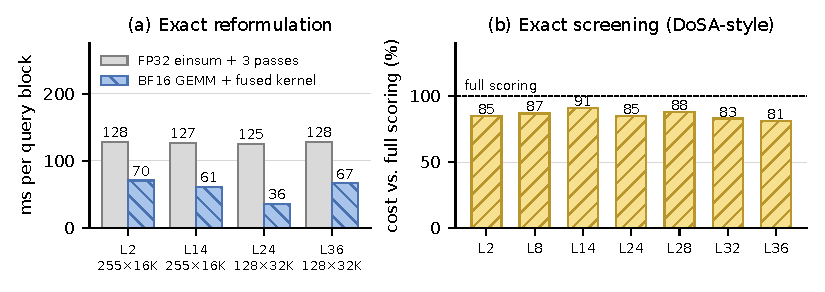
\includegraphics[width=\linewidth]{figures/indexer.pdf}
\caption{(a) Indexer time per prefill query block on real inputs, before and after the BF16 matmul and the fused head reduction. Labels give the layer and the block shape as rows times keys. Scores and selected keys are identical on these blocks. The matmul alone runs 1.5 to 1.9 times faster and the head reduction 5 to 6 times faster. (b) Cost of an exact screening bound relative to fully scoring the eligible keys, per index layer, at the best head budget. The bound was checked offline in float64 with slack for the BF16 roundings; the cost includes scoring the seed keys and is averaged over 17 queries of a 32K-token prompt with $K=512$.}
\label{fig:indexer}
\end{figure}
